% 
% Lecture Template for ME3050 -  Dynamics Modeling and Controls - Tennessee Technological University
%
% Tristan Hill, May 07, 2020 - June 12, 2020, % Spring 2020 - Summer 2020
% Module 7 - Damping Elements
% Topic 3 - Mass Spring Damper Model
%

\documentclass{beamer}                         % for presentation (has nav buttons at bottom)
%\documentclass[handout]{beamer}  % for handout 
\usepackage{beamerthemesplit}
\usepackage{amsmath}
\usepackage{bm}
\usepackage{listings}
\usepackage{multicol}
\usepackage{framed}

\beamertemplateballitem

% custom colors
\definecolor{TTUpurple}{rgb}{0.3098, 0.1607, 0.5176} % TTU Purple (primary)
\definecolor{TTUgold}{rgb}{1.0000, 0.8666, 0.0000} % TTU Gold (primary) 
\definecolor{mygray}{rgb}{.6, .6, .6}
\definecolor{mypurple}{rgb}{0.6,0.1961,0.8}
\definecolor{mybrown}{rgb}{0.5451,0.2706,0.0745}
\definecolor{mygreen}{rgb}{0, .39, 0}
\definecolor{mypink}{rgb}{0.9960, 0, 0.9960}

% color commands
\newcommand{\R}{\color{red}}
\newcommand{\B}{\color{blue}}
\newcommand{\BR}{\color{mybrown}}
\newcommand{\K}{\color{black}}
\newcommand{\G}{\color{mygreen}}
\newcommand{\PR}{\color{mypurple}}
\newcommand{\PN}{\color{mypink}}
\newcommand{\OR}{\color{TTU}}
\newcommand{\GD}{\color{TTUgold}}

% beamer colors
\setbeamercolor{palette primary}{bg=TTUpurple,fg=TTUgold}
\setbeamercolor{palette secondary}{bg=black,fg=TTUgold}
\setbeamercolor{palette tertiary}{bg=black,fg=TTUpurple}
\setbeamercolor{palette quaternary}{bg=TTUgold,fg=black}
\setbeamercolor{structure}{fg=TTUpurple} % itemize, enumerate, etc
\setbeamercolor{section in toc}{fg=TTUpurple} % TOC sections


\newcommand{\Lagr}{\mathcal{L}} % lagrangian

\newcommand{\hspcu}{\underline{\hspace{15mm}}} % large horizontal space w underline
\newcommand{\hspcuu}{\underline{\hspace{22mm}}} % larger horizontal space w underline

\newcommand{\vspccc}{\vspace{6mm}\\} % large vertical space
\newcommand{\vspcc}{\vspace{4mm}\\}   % medium vertical space
\newcommand{\vspc}{\vspace{2mm}\\}     % small vertical space

\newcommand{\hspcccc}{\hspace{10mm}} % large horizontal space
\newcommand{\hspccc}{\hspace{6mm}} % large horizontal space
\newcommand{\hspcc}{\hspace{4mm}}   % medium horizontal space
\newcommand{\hspc}{\hspace{2mm}}     % small horizontal space

\newsavebox{\mybox} % custom box


\newcommand{\MNUM}{7\hspace{2mm}} % Module number
\newcommand{\TNUM}{3\hspace{2mm}} % Topic number 
\newcommand{\moduletitle}{Damping Elements} % Titles and Stuff
\newcommand{\topictitle}{Mass Spring Damper Model} 

\newcommand{\sectiontitleI}{Standard Model Form} % More Titles and Stuff
\newcommand{\sectiontitleII}{Engineering Applications}
\newcommand{\sectiontitleIII}{Example: Automobile Suspension}
\newcommand{\sectiontitleIV}{---}

\author{ME3050 - Dynamics Modeling and Controls}
\title{Module \MNUM - \moduletitle}
\date{Mechanical Engineering\vspc Tennessee Technological University}

\begin{document}

\lstset{language=MATLAB,basicstyle=\ttfamily\small,showstringspaces=false}

\frame{\titlepage \center\begin{framed}\Large \textbf{Topic \TNUM - \topictitle}\end{framed} \vspace{5mm}}

% Section 0 - Outline
\frame{
	
	\large \textbf{Topic \TNUM - \topictitle} \vspace{3mm}\\
	
	\begin{itemize}
	
		\item \sectiontitleI    \vspc % Section I
		\item \sectiontitleII 	\vspc % Section II
		\item \sectiontitleIII 	\vspc %Section III
%		\item \sectiontitleIV 	\vspc %Section IV
	
	\end{itemize}

}

% Section I
\section{\sectiontitleI}

	% Section I - Frame I
	\frame{
		\frametitle{\sectiontitleI}
		
		The EOMs we have derived can be represented in the following standard form. \\
	%		\begin{framed}
		\[a_n\frac{d^n}{dt^n}x(t)+a_{n-1}\frac{d^{n-1}}{dt^{n-1}}x(t)+...+a_2\frac{d^2}{dt^2}x(t)+a_1\frac{d}{dt}x(t)+a_0x(t)=f(t)\] \vspc		
	%		\end{framed}
		
		\begin{itemize}
			\item The dependent variable $x$ and its derivatives depend on $t$. \vspc 
			\item The coefficients $a_n$ through $a_0$ are functions of the physical parameters in the system.
			\item The function f(t) is called the \hspcuu \hspc \hspcuu
			\item The system is linear if ...
		\end{itemize}

	}
	
	% Section I - Frame II
	\frame{
		\frametitle{\sectiontitleI}
		
		In solid mechanics and dynamics the standard form of the model becomes the generalized mass spring damper model. \vspc
		
			\[ a_nx^{(n)}+a_{n-1}x^{(n-1)}+...+a_{2}x''+a_{1}x'+a_0x=f(t) \] \\
			\[ \rightarrow \hspccc m\ddot{x}+c\dot{x}+k\dot{x}=f(t) \hspc \rightarrow \hspc {\bm M}\ddot{\bf x} +{\bm C}\dot{x}+{\bm K}\dot{x}={\bm f}(t)\]\vspc
			
		This is a fundamental equation that we will investigate throughout the rest of the semester.

	}

% Section II
\section{\sectiontitleII}
	
	% Section II - Frame I
	\frame{
		\frametitle{\sectiontitleII}

		The mass spring damper model can be applied to most mechanics problems.

		\begin{itemize}
			\item
			
			\item
			
			\item
		\end{itemize}


	}\Large


% Section III
\section{\sectiontitleIII}
	
		% Section III - Frame I
	\frame{ \small
		\frametitle{\sectiontitleIII}
		\begin{multicols}{2}
		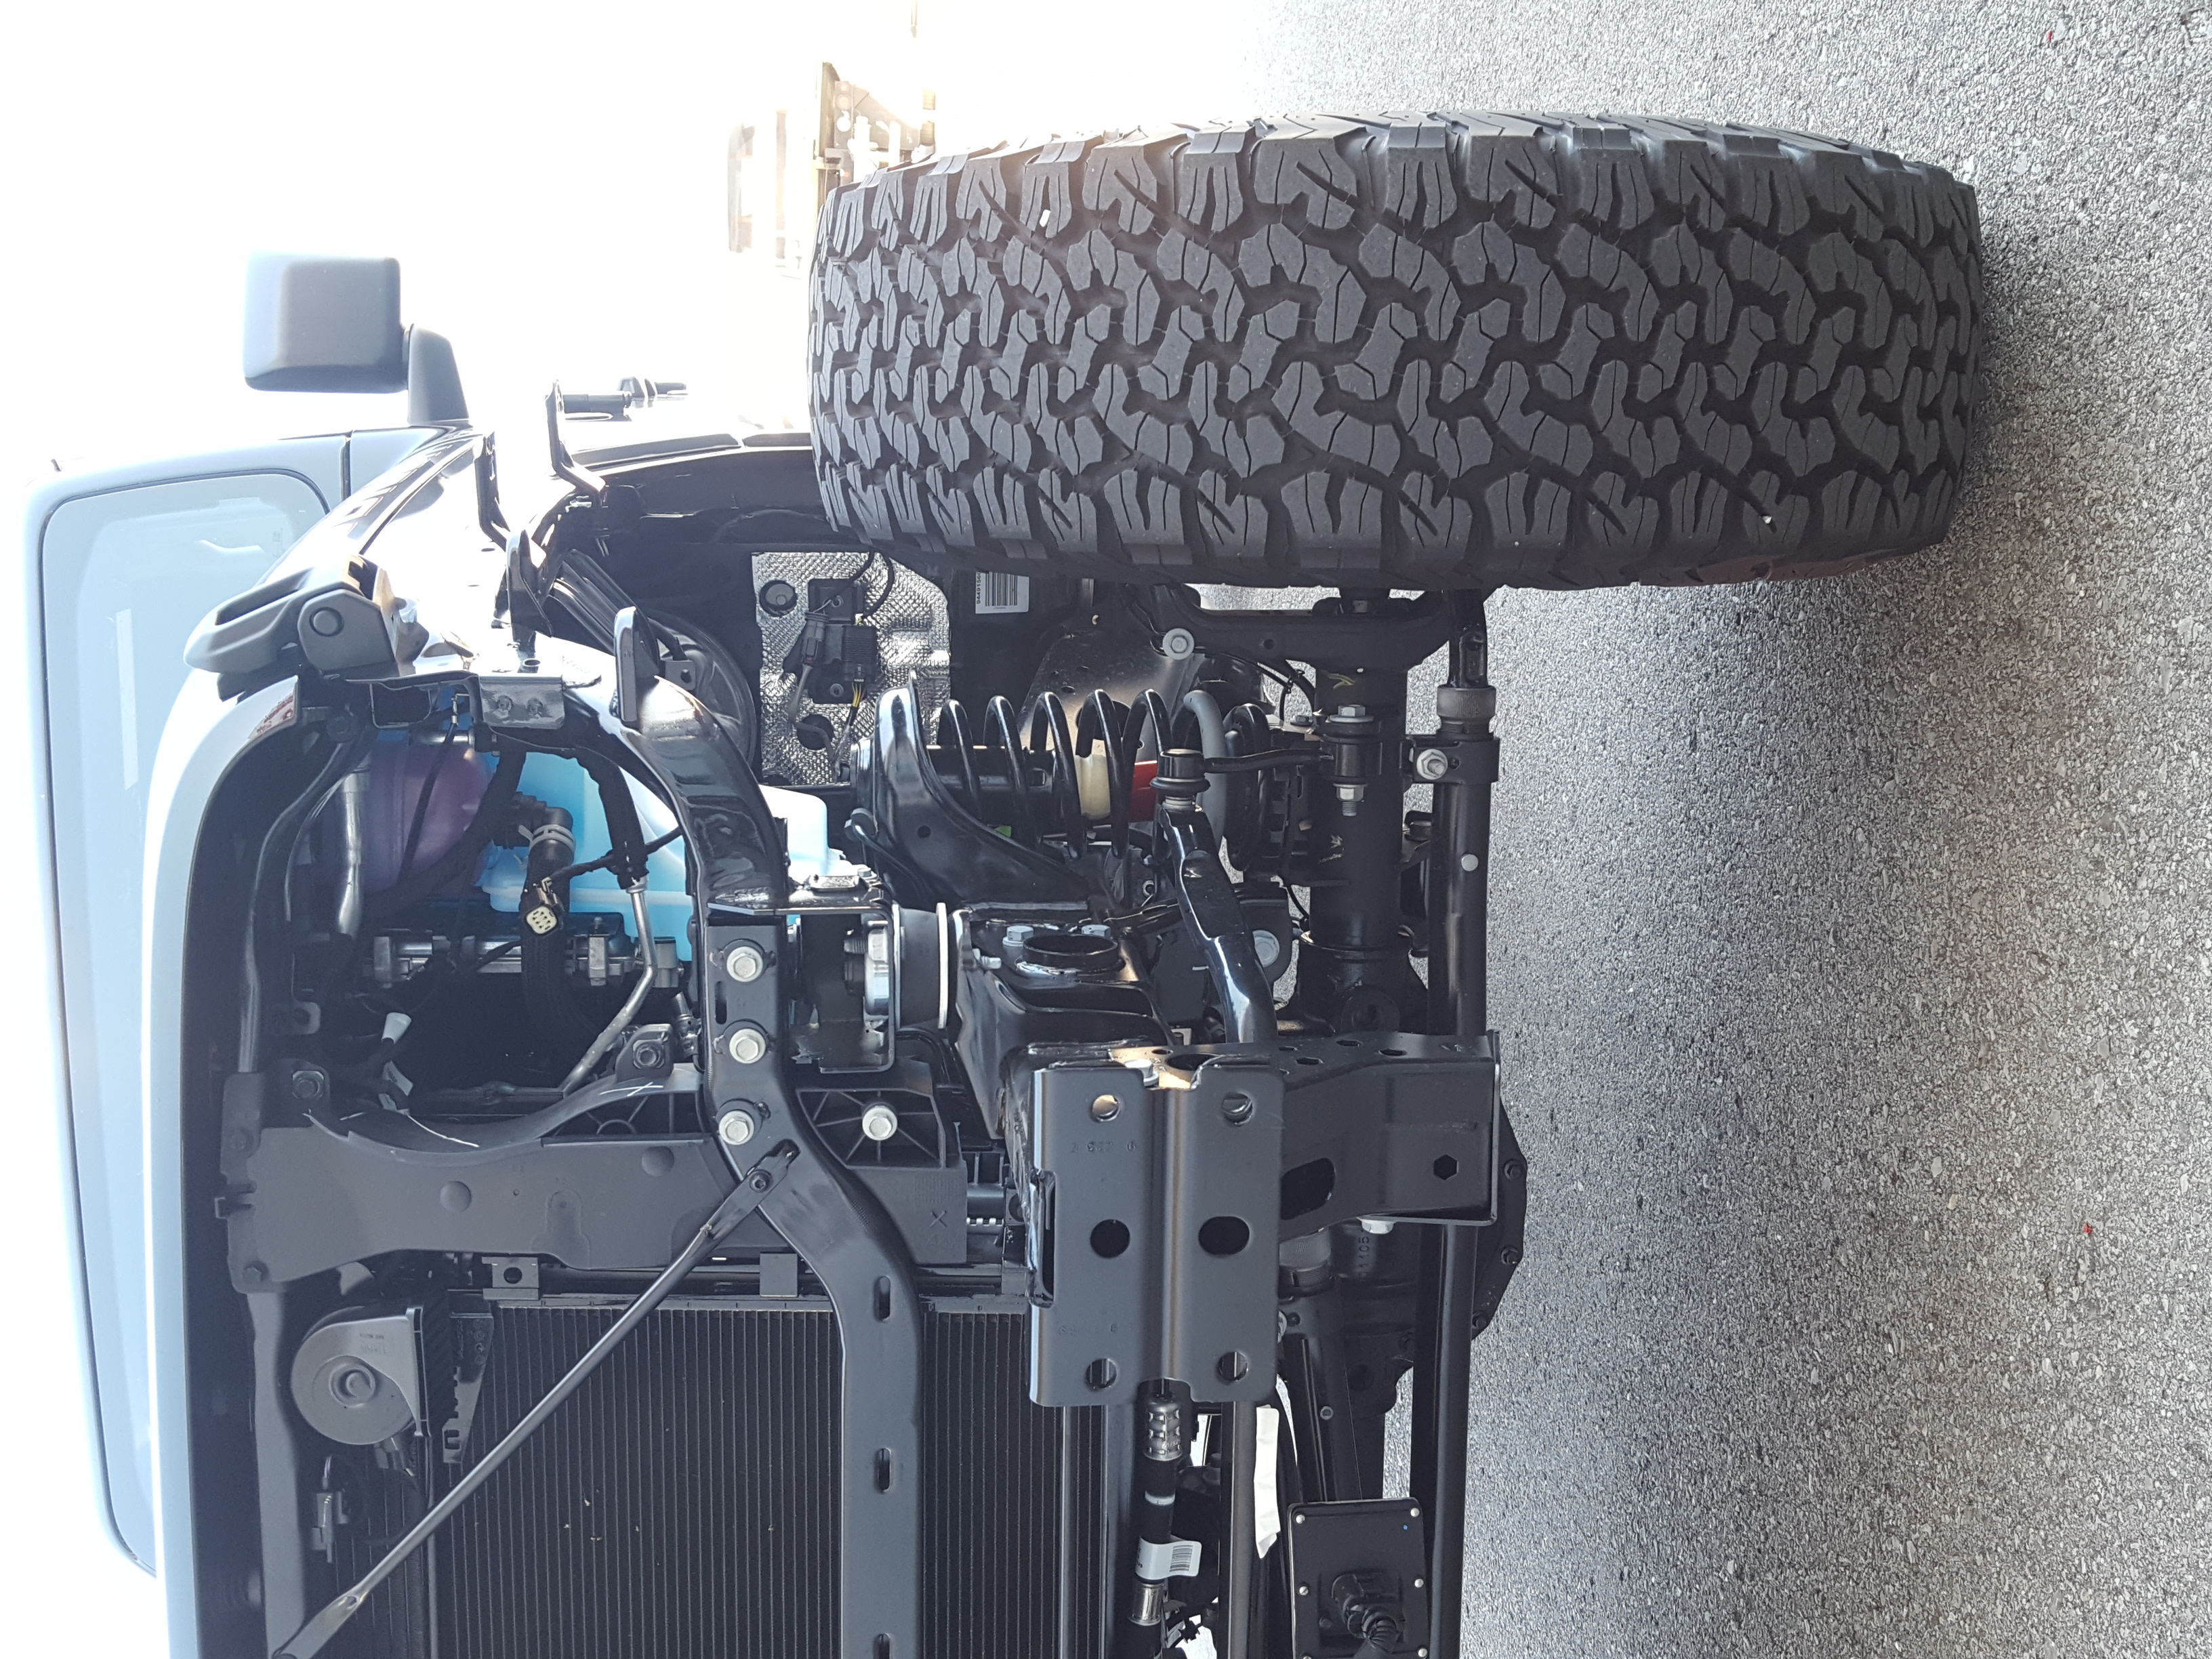
\includegraphics[scale=.05,angle=-90,origin=c]{jeep_01.jpg}	
		
		\textbf{  \underline{Newton's Second Law Approach} }\\
		\begin{enumerate}
			\item Draw a {\BR Free Body Diagram}
			\item Make an {\G assumption of motion}
			\item Determine all {\B forces} acting on the system and their {\B directions}. 
			\item Write {\PR Newton's second law} for the appropriate DOF. 
			\item Re-write the ODE in the {\PN standard form} of a system equation.
		\end{enumerate}

		\end{multicols}
	}
	
	% Section III - Frame II	
	\frame{
		\frametitle{\sectiontitleIII \hspace{1mm} - Steps 1,2 and 3}
		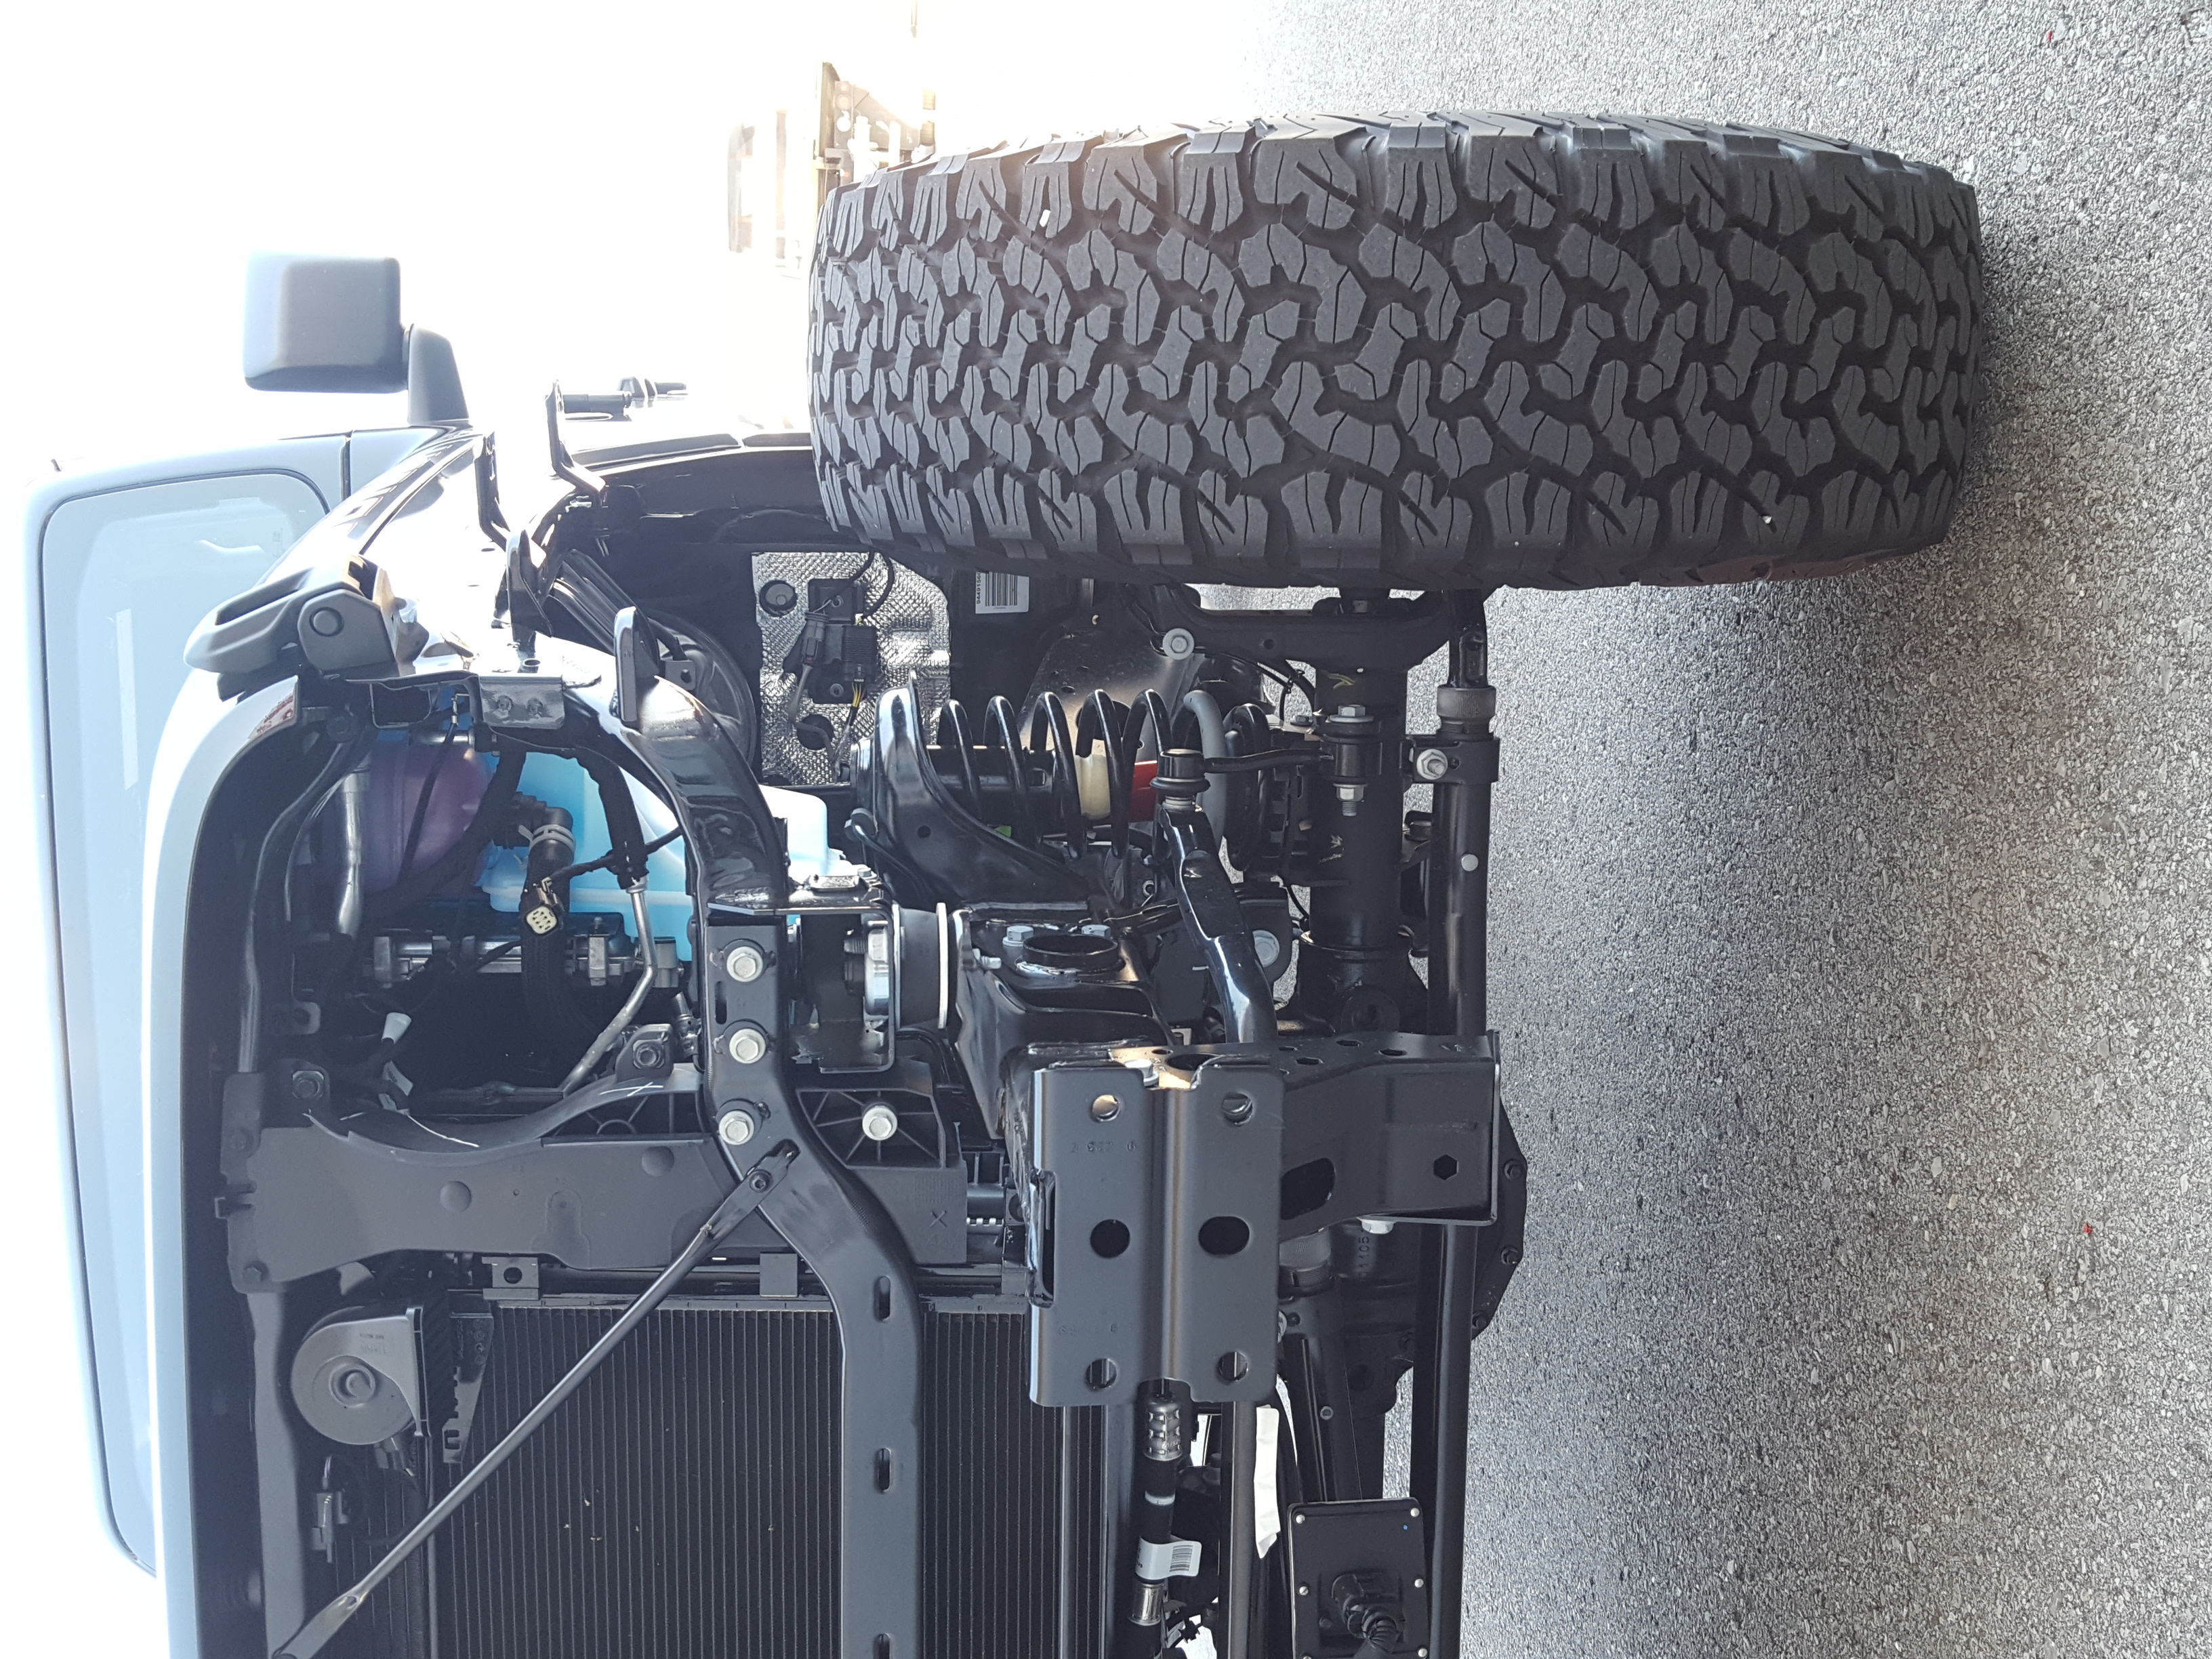
\includegraphics[scale=.05,angle=-90,origin=c]{jeep_01.jpg}	
	}
	
	% Section III - Frame III		
	\frame{
		\frametitle{\sectiontitleIII \hspace{1mm} - Steps 4,5}
		
	}	
	% Section III - Frame IV		
	\frame{
		\frametitle{---}
		
	}	
	% Section II - Frame V		
	\frame{
		\frametitle{---}
		
	}	
		
%% Section IV
%\section{\sectiontitleIV}
%	
%	% Section IV - Frame I
%	\frame{
%		\frametitle{\sectiontitleIV}
%		
%		
%	}
%	


	
\end{document}	
	
	
\end{document}




